\section{Case Studies and Evaluation}

In the following two sections, we evaluate SWiM 0.2 and a prototype based on Semantic
MediaWiki for their applicability to Flyspeck with regard to their support for
annotations, browsing, and querying, as specified in section~\ref{sec:req}.  For the case
study, we had the {\TeX} sources of the Flyspeck book and a Twelf formalization of the
first chapter (Trigonometry) at our disposal.\ednote{@Sean/Florian: One/two sentences
  about Twelf! (in some other section, either workflow or flyspeck)}

Both systems are semantic wikis, where one resource (in the RDF sense)---e.\,g.\ one
mathematical theorem---is represented by one wiki page and relations between resources by
links between pages.  Both pages and links can be typed with terms from
ontologies~\cite{OrDeMoVoHa06:annotation-navigation-semwiki}, which are either preloaded
into the wiki or modelled ad-hoc~\cite{KrSchVr:semwiki-reasoning07}.  This is the
prevalent approach of adding semantics to wikis, although other ways have been
investigated~\cite{semwiki06}.  Semantic wikis commonly offer enhanced navigation
capabilities by displaying a summary of all typed links, grouped by type, with each page.
Most of them allow to search for pages by type or by them being subject or object of any
RDF triple (= typed link), while it depends on the reasoner used by the wiki whether only
explicit RDF triples or also inferred ones are
considered~\cite{KrSchVr:semwiki-reasoning07}.  Such queries can usually be executed
interactively via a special search form, or in an automated way as \emph{inline} queries
embedded into the content of a page.  Except for interactive triple search not yet being
supported by SWiM, both systems support this basic set of semantic wiki features.

\subsection{SWiM 0.2}
\label{sec:swim}

SWiM is a semantic wiki for mathematical knowledge management.  Based on the
general-purpose semantic wiki IkeWiki~\cite{KrSchVr:semwiki-reasoning07}, it adds support
for browsing, editing, rendering, importing and exporting mathematical documents written
in OMDoc.  The semantics of mathematical knowledge is mainly captured in a \emph{document
  ontology}: Whenever a wiki page containing OMDoc fragments is stored, its type and its
(typed) relations to other items of mathematical knowledge in the wiki are extracted from
the OMDoc XML markup and explicitly represented as RDF triples in terms of the OMDoc
document ontology~\cite{OMDocDocOnto:web}.  This ontology models those aspects of the
three layers of mathematical knowledge supported by OMDoc to the extent supported by the
expressivity of OWL-DL.  Modeling all modules of the OMDoc specification in this ontology
is work in progress; so far, most mathematical statements as well as key aspects of
theories have been implemented.  Relevant classes for Flyspeck would be
\textit{Lemma}/\textit{Theorem}/\textit{Corollary}/\ldots (all being subclasses of
\textit{Assertion}), \textit{Proof}, \textit{Symbol} (a symbol declaration),
\textit{Definition}, and the properties \textit{Proof--proves--Assertion} and
\textit{Symbol--hasDefinition--Definition}.  Dependencies can partly be inferred by a DL
reasoner, but for a complete support of OMDoc's notion of dependency, an OMDoc-specific
calculus will have to be applied, which is currently in development.

\begin{figure}
  \centering
  \begin{tikzpicture}[set style={{default}+=[scale=.47,font=\normalsize\sffamily]},default]
    \tikzstyle{every path}=[font=\small\sffamily];
    \node[concept] (s) at (0,0) {\itshape Statement};
    \node[concept] (d) at (-7.5,-3) {Definition};
    \node[concept] (y) at (-2.5,-3) {Symbol};
    \node[concept] (a) at (+2.5,-3) {Assertion};
    \node[concept] (p) at (+7.5,-3) {Proof};

    \node[concept] (l) at (-1.5,-6) {Lemma};
    \node[concept] (c) at (+2.5,-6) {Corollary};
    \node[concept] (t) at (+6.5,-6) {Theorem};

    \draw[-open triangle 60] (y) -- (s);
    \draw[-open triangle 60] (d) -- (s);
    \draw[-open triangle 60] (a) -- (s);
    \draw[-open triangle 60] (p) -- node[right=1ex] {$\sqsubseteq$} (s);

    \draw[-open triangle 60] (l) -- (a);
    \draw[-open triangle 60] (c) -- (a);
    \draw[-open triangle 60] (t) -- (a);

    \draw[->] (d) -- node[below] {uses} (y);
    \draw[->] (a) -- node[below] {uses} (y);
    \draw[->] (p) -- node[below] {proves} (a);

    \draw[->] (s.0) .. controls +(0:2cm) and +(60:2cm)
    .. node[right=1pt,text width=2cm,text centered] (dep)
    {\itshape depends on} (s.60);

    \draw[->] (y.-120) .. controls +(-120:1cm) and +(-60:1cm) .. node[below] {hasDefinition} (d.-60);
  \end{tikzpicture}
  \caption{A relevant subset of the OMDoc document ontology}
  \label{fig:doconto}
\end{figure}

In the current version 0.2 of SWiM, the browsing of mathematical documents is powered by
the document ontology: Whenever RDF triples having the current page as subject or object
are available, most of them using terms from the OMDoc document ontology if the current
page is a mathematical document, they are displayed as navigation links (see
figure~\ref{fig:swim-lemma}).  Adding more ontology-powered services, particularly ones
that facilitate editing documents, is planned for version
0.3~\cite{swim-roadmap,Lange:SWiMSciColl07}.  Documents are presented as XHTML+MathML,
generated by the \textit{mmlkit} renderer~\cite{mmlkit:web}, with mathematical symbols
linked to their declarations.

\begin{figure}
  \centering
  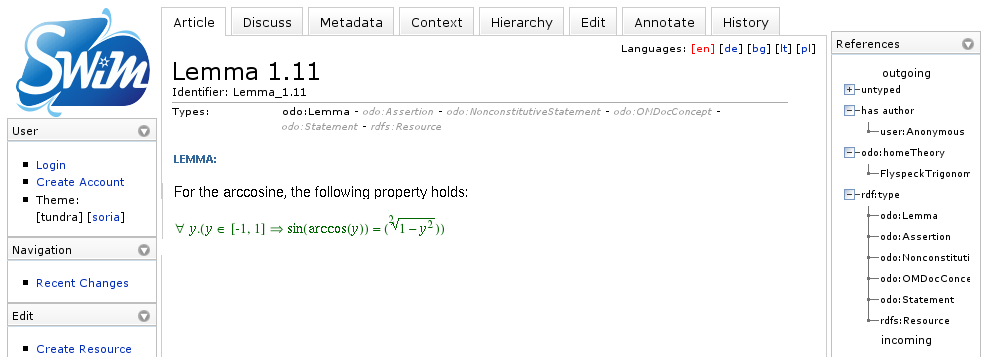
\includegraphics[width=.7\textwidth]{swim-lemma}
  \caption{A Flyspeck lemma in SWiM}
  \label{fig:swim-lemma}
\end{figure}

We manually recreated one Flyspeck lemma in SWiM and judged about the further annotation
capabilities from our previous experience with implementing SWiM and modeling other
document collections (as the OpenMath content dictionaries) in the system.\ednote{This is
  honest and really sufficient IMHO, but maybe sounds a bit weak -- what do you think?
  --CL} For testing a larger subset of Flyspeck, it would, however, have been possible to
convert the Twelf master source to OMDoc with our already existing converter, and to
import the generated OMDoc documents into SWiM using the built-in import functionality.
OMDoc would offer excellent support for the alternative workflow of stepwise formalization
as well~\cite[chap.\ 4]{Kohlhase:omdoc1.2}.  One could either start with converting the
Flyspeck book from {\LaTeX} to HTML with Presentation MathML and step by step formalize
the presentation markup into content markup, or one could start the formalization on the
{\TeX} side, using s\TeX{}, a content-oriented {\TeX} notation for OMDoc which can then be
converted to OMDoc~\cite{Kohlhase:albwo06}.

We found SWiM to be suitable for making Flyspeck browsable, as it supports breaking down
mathematical knowledge to the statement level and recognizes all required link types.  As
every SWiM page has an associated discussion page and discussion posts are semantically
represented using the SIOC ontology~\cite{SIOC:web}, one could also support the
coordination of the project by queries like query~\ref{item:question-count} from
section~\ref{sec:req}.  OMDoc markup and mathematical formulae in discussion pages are not
yet implemented, though.  Pages and non-OMDoc links can be annotated with types from
ontologies loaded into the wiki\footnote{Types of OMDoc links are automatically extracted
  from the markup; see above.}.  That means that the annotations required by Flyspeck can
be made, but not in an ad-hoc way, which we would have found useful in the prototyping
phase.  Instead, one would have to import an existing ontology into the wiki, or create it
using IkeWiki's ontology editor---SWiM supports both---, and then one would be able to
annotate documents using terms from that ontology.

Searching for arbitrary RDF triples is not yet supported by the user interface,
but authors can embed inline SPARQL queries into wiki pages.  Note that not all desirable
queries are easy to express in SPARQL; consider query~\ref{item:proven-lemma}:

\begin{lstlisting}
SELECT ?l WHERE { ?l rdf:type odo:Lemma .
                  ?l swrc:isAbout <Composite_Regions> .
                  OPTIONAL { ?p rdf:type odo:Proof .
                             ?p odo:proves ?l . }
                  FILTER ( ! bound(?p) ) }
\end{lstlisting}

This query assumes a SPARQL semantics with negation as failure~\cite{Polleres:SPARQL-Rules07}.  Alternatively, the query
can be made more intuitive by enhancing the ontology by the following concept:

\[
\mbox{LemmaWithoutProof}\equiv\mbox{Lemma}\sqcap\neg(\exists\mbox{proves}^{-1}.\mbox{Proof})
\]

The downloading part of the Flyspeck workflow is not yet natively supported by SWiM.
Currently, the only mathematical export format supported by SWiM is OMDoc, which could
then be converted to theorem proving languages by client-side software~\cite[chap.\
25.2]{Kohlhase:omdoc1.2}.

\subsection{Semantic MediaWiki 1.0}
\label{sec:smw-study}

Semantic MediaWiki~\cite{KrSchVr:semwiki-reasoning07} is a semantic web extension to
MediaWiki, the system driving Wikipedia.  Plain MediaWiki supports mathematical formulae
written in {\LaTeX} and allows for categorizing pages.  Semantic MediaWiki interprets
category membership as an instance-of relationship and adds the possibility to type links
and to create and edit these link types, called properties.  External ontologies can be
referenced from the wiki, but at most sites powered by Semantic MediaWiki, site-specific
ontologies are developed in an ad-hoc manner.  We found this useful while
\emph{prototyping} the annotations that might be required for Flyspeck, e.\,g.\
project-related metadata like the information whether a lemma has already been proven, or
categorization by topic.  It was less useful in places where ontologies already existed;
for structures of mathematical documents, it was just possible to reference
\emph{vocabulary} from the OMDoc document ontology, but not to do apply further inference
rules given there to items of mathematical knowledge, as Semantic MediaWiki does not
support a full \emph{import} of external ontologies.  Moreover, Semantic MediaWiki does
not understand the semantics of mathematical formulae, as the {\LaTeX} formulae cannot be
annotated.

In Semantic MediaWiki, we imported the Twelf master source of Flyspeck via a customly
implemented special page that uses the well-documented extension API of MediaWiki.  The
Twelf file was first enhanced by special comment lines marking beginning and end of a
declaration\ednote{@Sean/Florian: What's the general term?} with information about topical
categorization.  The Twelf upload extension breaks an uploaded file down into declarations
and creates two wiki pages for each Twelf declaration: one page that just contains the
Twelf listing, categorized in its respective category of the OMDoc document ontology
(e.\,g.\ \textit{Lemma}), and one container page that includes the Twelf page via
MediaWiki's template inclusion mechanism, but also allows for including a {\LaTeX}
representation and leaving space for free-form annotations made by the contributors step
by step.  The Twelf pages are overwritten on every import from the master source, whereas
existing container pages remain untouched.

For typing knowledge items, we used a simple-minded syntax-driven approach of encoding the
type in the identifier of the declaration; the identifier of a lemma would start with
``lemma-''.  We could also have employed Twelf's inference to determine the
type\ednote{@Florian: Reword this correctly!}, as our Twelf-to-OMDoc converter does.
Additionally, the upload extension recognizes all previously imported symbols in Twelf
expressions and turns them into links of the type \textit{\ldots--uses--Symbol}.

\begin{figure}
  \centering
  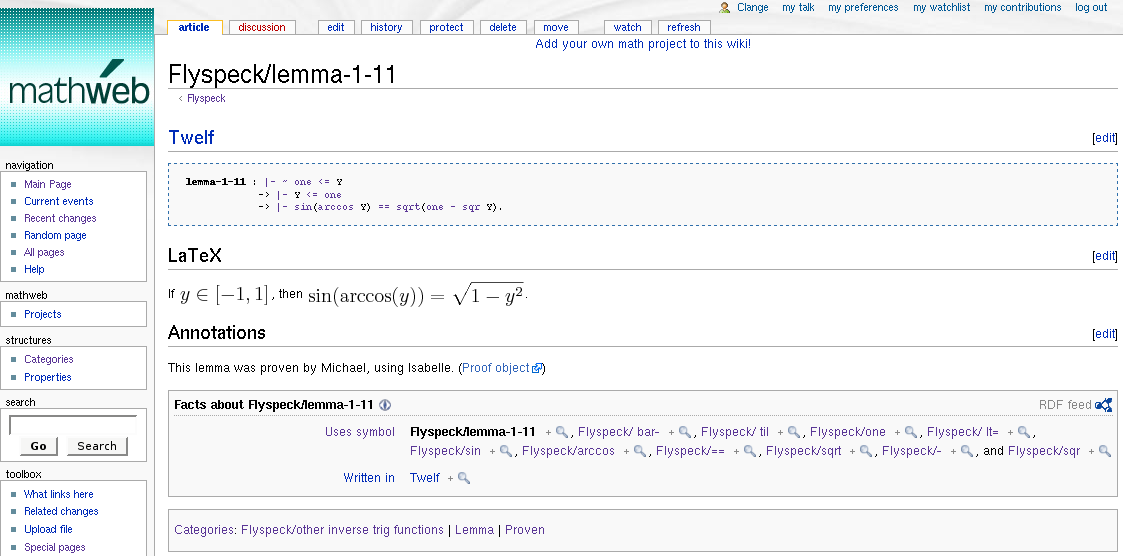
\includegraphics[width=\textwidth]{smw-lemma}
  \caption[A Flyspeck lemma in Semantic MediaWiki]{A Flyspeck lemma in Semantic
    MediaWiki\protect\footnotemark}
  \label{fig:smw-lemma}
\end{figure}
\addtocounter{footnote}{-1}
\stepcounter{footnote}\footnotetext{See \url{http://mathweb.org/wiki/Flyspeck}}

The annotations generated that way can be used for browsing, either via the summary of all
typed links in the ``fact box'', or by the special ``browse'' page.  For querying,
Semantic MediaWiki offers a simple triple search, as well as inline queries.  The latter
are intuitive to write but less powerful than SPARQL queries on an RDF store using an
OWL-DL reasoner; the query language corresponds to the description logic
$\mathcal{EL}^{++}$~\cite{KrSchVr:semwiki-reasoning07}, which, for example, does not
support negation.  A query for proven lemmas about a certain topic that have a Twelf
representation would be written as follows:

\begin{lstlisting}
<ask>[[Category:Proven]] [[Category:Lemma]]
     [[Category:Trigonometry]] [[written in::Twelf]]</ask>
\end{lstlisting}

Here, most annotations are modelled by categorization, i.\,e.\ instantiation of
classes---certainly not the most formal way of structuring knowledge in view of many
classes just corresponding to narrative sections of the book, but the one that is
supported best by Semantic MediaWiki.  More complex reasoning tasks like inference of
dependencies are not possible in Semantic MediaWiki; in this domain-specific setting one
could realize them by hard-coded extension functions.

Exporting formal representations of knowledge items is not yet supported conveniently.
The Twelf listings can be viewed on their own pages, but due to the auto-generated symbol
links in the source code, these are not suitable for download.  One would either have to
implement a special Twelf download page that cleans these sources again, or one would have
to implement the symbol linking as an extension of the rendering process.

%%% Local Variables: 
%%% mode: latex
%%% TeX-master: "flyspeck-wiki-eswc08"
%%% End: 
